\chapter{SISTEM JARINGAN}

Sistem jaringan yang nantinya dibangun akan terlihat seperti pada gambar \ref{fig:network-dia} berikut ini :

\begin{figure}[H]
	\centering
	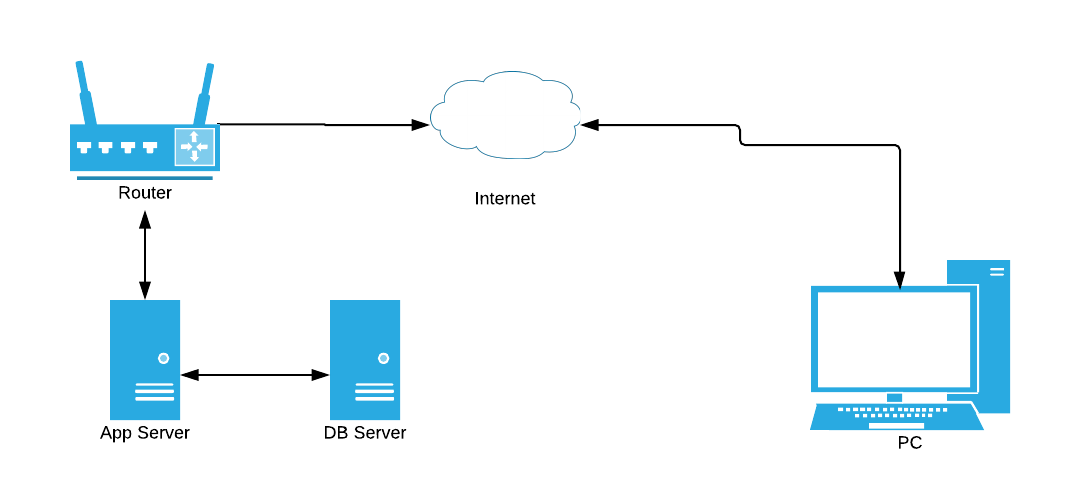
\includegraphics[width=1\textwidth]{./resources/network-diagram}
	\caption{Diagram Sistem Jaringan Sistem Informasi PBB-P2}
	\label{fig:network-dia}
\end{figure}

Diagram tersebut menggambarkan bahwa peladen aplikasi akan berkomunikasi atau berhubungan langsung dengan peladen sistem basis data apabila ada permintaan data yang terjadi.

Untuk menghubungkan peladen aplikasi dengan dunia luar (internet) agar dapat diakses oleh masyarakat wajib pajak, maka diperlukan \textit{router} yang akan menghubungkan jaringan lokal dengan jaringan internet.

Dari jaringan internet inilah masyarakat wajib pajak dapat melakukan akses ke aplikasi dan memperoleh informasi pembayaran tahun berapa saja yang menjadi hutang yang belum terbayar, dan pada tahun berapa saja yang sudah dilunasi.

Masyarakat wajib pajak pun dapat melihat informasi terkini mengenai data subjek pajak dan data objek pajak terbaru.